%%%%%%%%%%%%%%%%%%%%%%%%%%%%%%%%%%%%%%%%%
% Jacobs Landscape Poster
% LaTeX Template
% Version 1.0 (29/03/13)
%
% Created by:
% Computational Physics and Biophysics Group, Jacobs University
% https://teamwork.jacobs-university.de:8443/confluence/display/CoPandBiG/LaTeX+Poster
% 
% Further modified by:
% Nathaniel Johnston (nathaniel@njohnston.ca)
%
% This template has been downloaded from:
% http://www.LaTeXTemplates.com
%
% License:
% CC BY-NC-SA 3.0 (http://creativecommons.org/licenses/by-nc-sa/3.0/)
%
%%%%%%%%%%%%%%%%%%%%%%%%%%%%%%%%%%%%%%%%%

%----------------------------------------------------------------------------------------
%	PACKAGES AND OTHER DOCUMENT CONFIGURATIONS
%----------------------------------------------------------------------------------------

\documentclass[final]{beamer}

\usepackage[scale=1.24]{beamerposter} % Use the beamerposter package for laying out the poster

\usetheme{confposter} % Use the confposter theme supplied with this template

\setbeamercolor{block title}{fg=ngreen,bg=white} % Colors of the block titles
\setbeamercolor{block body}{fg=black,bg=white} % Colors of the body of blocks
\setbeamercolor{block alerted title}{fg=white,bg=dblue!70} % Colors of the highlighted block titles
\setbeamercolor{block alerted body}{fg=black,bg=dblue!10} % Colors of the body of highlighted blocks
% Many more colors are available for use in beamerthemeconfposter.sty

%-----------------------------------------------------------
% Define the column widths and overall poster size
% To set effective sepwid, onecolwid and twocolwid values, first choose how many columns you want and how much separation you want between columns
% In this template, the separation width chosen is 0.024 of the paper width and a 4-column layout
% onecolwid should therefore be (1-(# of columns+1)*sepwid)/# of columns e.g. (1-(4+1)*0.024)/4 = 0.22
% Set twocolwid to be (2*onecolwid)+sepwid = 0.464
% Set threecolwid to be (3*onecolwid)+2*sepwid = 0.708

\newlength{\sepwid}
\newlength{\onecolwid}
\newlength{\twocolwid}
\newlength{\threecolwid}
\setlength{\paperwidth}{48in} % A0 width: 46.8in
\setlength{\paperheight}{36in} % A0 height: 33.1in
\setlength{\sepwid}{0.024\paperwidth} % Separation width (white space) between columns
\setlength{\onecolwid}{0.22\paperwidth} % Width of one column
\setlength{\twocolwid}{0.464\paperwidth} % Width of two columns
\setlength{\threecolwid}{0.708\paperwidth} % Width of three columns
\setlength{\topmargin}{-0.5in} % Reduce the top margin size
%-----------------------------------------------------------

\usepackage{graphicx}  % Required for including images
\usepackage{booktabs} % Top and bottom rules for tables
\usepackage{amsmath,amsfonts,amssymb}
\usepackage{bm}
\usepackage{multirow}
\usepackage{makecell}


% bold x for equations
\newcommand{\rmx}{\mathrm x} 
% used for table headers
\newcommand{\tabh}[1]{\multicolumn{1}{c}{\textbf{#1}}}  
\newcommand{\tabhr}[1]{\multicolumn{1}{c}{\textbf{#1}}}  
% used for the top left cell in a table
\newcommand{\tabc}[2]{\multicolumn{1}{c}{\multirow{#1}{*}{\textbf{#2}}}} 
% used for denoting the loss symbol with a subscript
\newcommand{\loss}[1]{J_{\text{#1}}}
% used for denoting the lambda symbol with a subscript
\newcommand{\hyp}[1]{\lambda_{\text{#1}}}
% used for denoting the theta symbol with a subscript
\newcommand{\nnweight}[1]{\bm{\theta_{\text{#1}}}}
% used for denoting the weight symbol (w) with a subscript
\newcommand{\weight}[1]{W_{\text{#1}}}
% used for denoting the bias symbol (b) with a subscript
\newcommand{\bias}[1]{\bm{b_{\text{#1}}}}

%----------------------------------------------------------------------------------------
%	TITLE SECTION 
%----------------------------------------------------------------------------------------

\title{Disentangled Representation Learning for Non-Parallel Text Style Transfer} % Poster title

\author{Vineet John, Lili Mou, Hareesh Bahuleyan and Olga Vechtomova} % Author(s)

\institute{University of Waterloo} % Institution(s)

%----------------------------------------------------------------------------------------

\begin{document}

\graphicspath{{images/}}

\addtobeamertemplate{block end}{}{\vspace*{2ex}} % White space under blocks
\addtobeamertemplate{block alerted end}{}{\vspace*{2ex}} % White space under highlighted (alert) blocks

\setlength{\belowcaptionskip}{2ex} % White space under figures
\setlength\belowdisplayshortskip{2ex} % White space under equations

\begin{frame}[t] % The whole poster is enclosed in one beamer frame

    \begin{columns}[t] % The whole poster consists of three major columns, the second of which is split into two columns twice - the [t] option aligns each column's content to the top

        \begin{column}{\sepwid}\end{column} % Empty spacer column

        \begin{column}{\onecolwid} % The first column

            %----------------------------------------------------------------------------------------
            %	OBJECTIVES
            %----------------------------------------------------------------------------------------

            \begin{alertblock}{Objectives}

                \begin{itemize}
                    \item Disentangle the latent representations of style and content in language models
                    \item Use the disentangled model to transfer text attributes and generate new sentences
                \end{itemize}

            \end{alertblock}

            %----------------------------------------------------------------------------------------
            %	INTRODUCTION
            %----------------------------------------------------------------------------------------

            \begin{block}{Introduction}

                In this paper, we address the problem of disentangling the latent space of neural networks for text generation.
                Our model is built on an autoencoder that encodes a sentence to the latent space (vector representation) by learning to reconstruct the sentence itself.

                To accomplish this, we propose a simple yet effective approach that combines multi-task and adversarial objectives.
                We artificially divide the latent representation into two parts: the style space and content spaces.
                We then use a multi-task loss that operates on a latent space to ensure that the space does contain the information we wish to encode.
                The adversarial loss, on the contrary, minimizes the predictability of information that should not be contained in a given latent space.

                A direct application of our disentangled latent space is style-transfer sentence generation, i.e., we can synthesize a sentence with generally the same meaning but a different style in the inference stage.

            \end{block}

            %------------------------------------------------

            \begin{figure}
                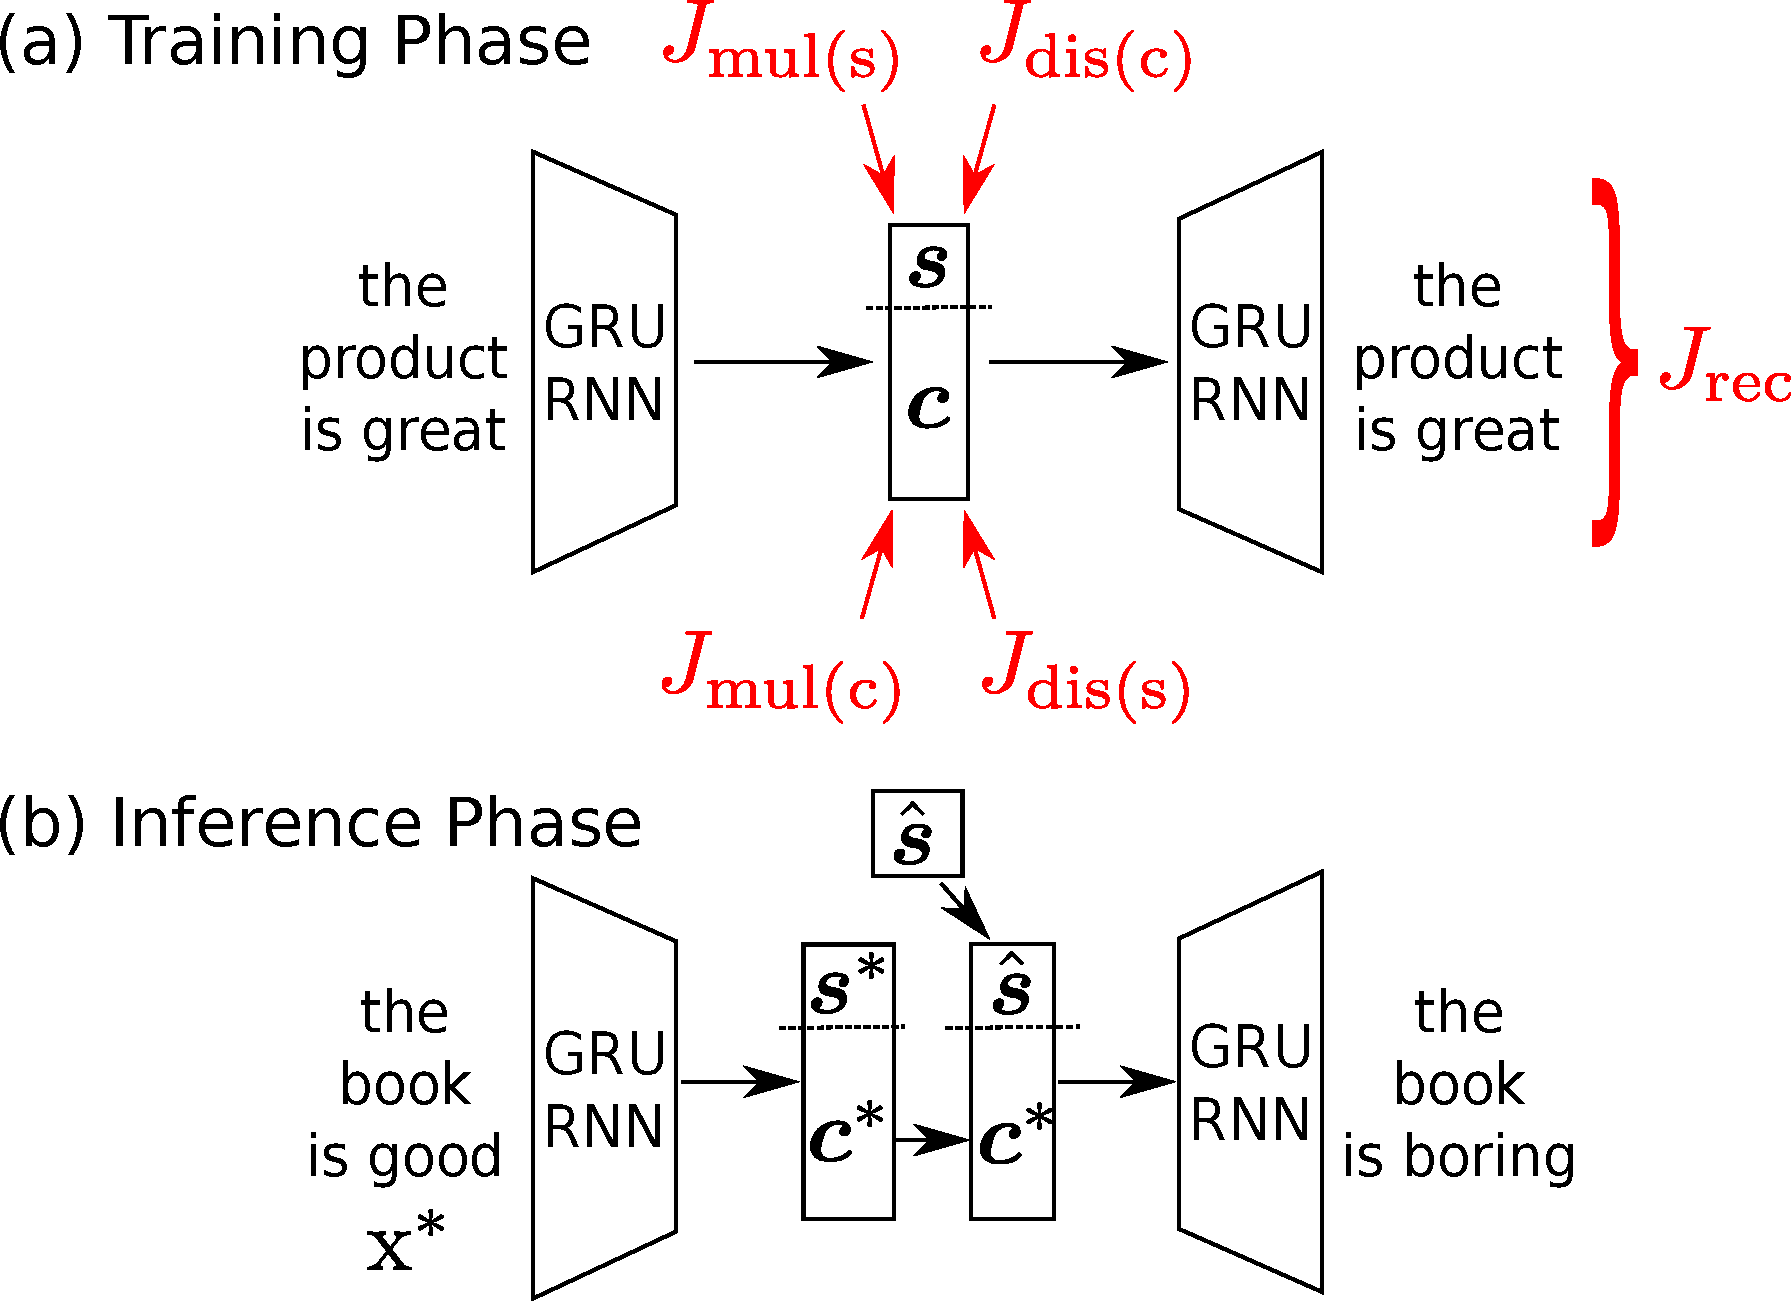
\includegraphics[width=1\linewidth]{model-overview}
                \caption{Model Training and Inference}
            \end{figure}

            %----------------------------------------------------------------------------------------

        \end{column} % End of the first column

        \begin{column}{\sepwid}\end{column} % Empty spacer column

        \begin{column}{\twocolwid} % Begin a column which is two columns wide (column 2)

            \begin{columns}[t,totalwidth=\twocolwid] % Split up the two columns wide column

                \begin{column}{\onecolwid}\vspace{-.6in} % The first column within column 2 (column 2.1)

                    %----------------------------------------------------------------------------------------
                    %	MATERIALS
                    %----------------------------------------------------------------------------------------

                    \begin{block}{Model}

                        The \textbf{VAE \cite{kingma2013auto} reconstruction loss} is
                        \begin{align*}
                            \loss{AE}(\nnweight{E}, \nnweight{D}) = & - \mathbb{E}_{q_{E}(\bm h|\rmx)} [\log p(\rmx|\bm h)]    \\
                                                                    & + \hyp{kl}\operatorname{KL}(q_{E}(\bm h|\rmx)\|p(\bm h))
                        \end{align*}
                        where $\hyp{kl}$ is the hyperparameter balancing the reconstruction loss and the KL term. $p(\bm h)$ is the prior, typically the standard normal  $\mathcal{N}(\bm 0,\mathrm I)$. $q_E(\bm h|\mathrm x)$ is the posterior in the form $\mathcal{N}(\bm \mu,\operatorname{diag} \bm\sigma^2)$, where $\bm\mu$ and $\bm\sigma$ are predicted by the encoder.

                        The \textbf{multi-task classifier} loss is given by
                        \begin{equation*}
                            \bm y_s = \operatorname{softmax}(\weight{mul(s)} \bm s + \bias{mul(s)})
                        \end{equation*}
                        where $\nnweight{mul(s)}=[\weight{mul(s)}; \bias{mul(s)}]$ are the parameters of the style classifier in the setting of multi-task learning, and $\bm y_s$ is the output of softmax layer.
                        The classifier is trained with cross-entropy loss against the ground-truth distribution.

                    \end{block}

                    %----------------------------------------------------------------------------------------

                \end{column} % End of column 2.1

                \begin{column}{\onecolwid}\vspace{-.6in} % The second column within column 2 (column 2.2)

                    %----------------------------------------------------------------------------------------
                    %	METHODS
                    %----------------------------------------------------------------------------------------

                    \begin{block}{Model (contd.)}
                        We train an \textbf{adversarial classifier}, that deliberately discriminates the style label.
                        Then, the encoder is trained to encode a content space from which its adversary cannot predict the style.
                        \begin{equation*}
                            \bm y_s                          = \operatorname{softmax}(\weight{dis(s)} \bm c + \bias{dis(s)})
                        \end{equation*}
                        \begin{equation*}
                            \loss{dis(s)}(\nnweight{dis(s)}) = - \sum\nolimits_{l\in\text{labels}} t_c(l)\log y_s(l)
                        \end{equation*}
                        where $\nnweight{dis(s)}=[\weight{dis(s)}; \bias{dis(s)}]$ are the parameters of the adversary.

                        The style-oriented adversarial objective maximizes
                        \begin{equation*}
                            \loss{adv(s)}(\nnweight{E})=\mathcal{H}(\bm y_s|\bm c; \nnweight{dis(s)})
                        \end{equation*}
                        where $\bm y_s$ is the predicted distribution over the style labels and $\mathcal{H}(\bm p)=-\sum_{i\in\text{labels}}p_i\log p_i$ is the entropy of the adversary. Here, $\loss{adv(s)}$ is maximized with respect to the encoder $\nnweight{E}$ and we fix $\nnweight{dis(s)}$. The objective attains maximum value when $\bm y_s$ is uniform.

                    \end{block}

                    %----------------------------------------------------------------------------------------

                \end{column} % End of column 2.2

            \end{columns} % End of the split of column 2 - any content after this will now take up 2 columns width

            %----------------------------------------------------------------------------------------
            %	IMPORTANT RESULT
            %----------------------------------------------------------------------------------------

            % \begin{alertblock}{Important Result}

            %     We systematically combine multi-task and adversarial objectives to separate content and style from each other, where we also propose to approximate content information with bag-of-words features of style-neutral, non-stopword vocabulary.
            %     The disentangled space can be directly applied to text style-transfer tasks.
            %     Our method achieves high style-transfer strength, high content-preservation scores, as well as high language fluency, compared with previous work.

            % \end{alertblock}

            %----------------------------------------------------------------------------------------

            \begin{columns}[t,totalwidth=\twocolwid] % Split up the two columns wide column again

                \begin{column}{\onecolwid} % The first column within column 2 (column 2.1)

                    %----------------------------------------------------------------------------------------
                    %	MATHEMATICAL SECTION
                    %----------------------------------------------------------------------------------------

                    \begin{block}{Results}

                    \end{block}

                    %----------------------------------------------------------------------------------------

                \end{column} % End of column 2.1

                \begin{column}{\onecolwid} % The second column within column 2 (column 2.2)

                    %----------------------------------------------------------------------------------------
                    %	RESULTS
                    %----------------------------------------------------------------------------------------

                    \begin{block}{Results (contd.)}

                        \begin{figure}
                            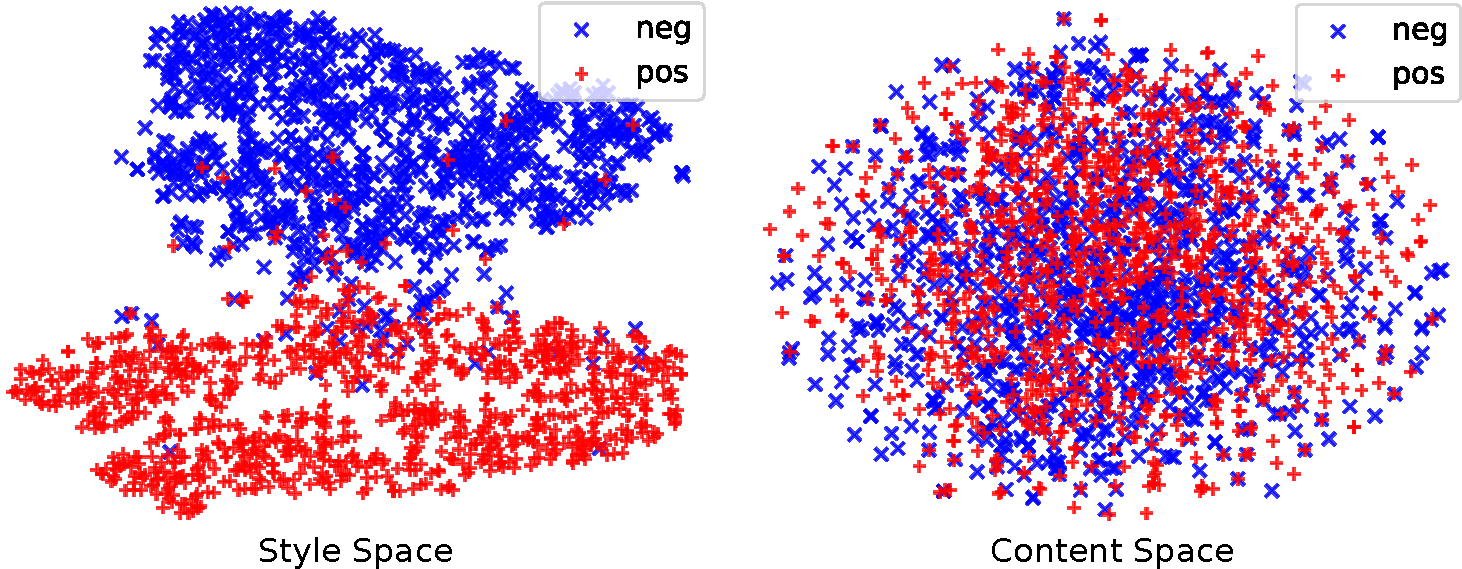
\includegraphics[width=\linewidth]{vae-latent-spaces}
                            \caption{Disentangled Latent Spaces - VAE}
                        \end{figure}

                        Table~\ref{tab:manual-evaluation} presents the results of human evaluation on selected methods.

                        \begin{table}[ht]
                            \centering
                            \begin{tabular}{ l c c c c }
                                \tabc{1}{Model} & \textbf{TS}       & \textbf{CP}       & \textbf{LQ}       & \textbf{GM}       \\
                                \hline
                                Fu (2018)       & \color{gray} 1.67 & \color{gray} 3.84 & \color{gray} 3.66 & \color{gray} 2.86 \\
                                Shen (2017)     & 3.63              & 3.07              & 3.08              & 3.25              \\
                                Zhao (2018)     & 3.55              & 3.09              & 3.77              & 3.46              \\
                                Ours (DAE)      & 3.67              & 3.64              & 4.19              & 3.83              \\
                                Ours (VAE)      & \textbf{4.32}     & \textbf{3.73}     & \textbf{4.48}     & \textbf{4.16}     \\
                            \end{tabular}
                            \caption{Manual evaluation on the Yelp dataset.}
                            \label{tab:manual-evaluation}
                        \end{table}

                    \end{block}

                    %----------------------------------------------------------------------------------------

                \end{column} % End of column 2.2

            \end{columns} % End of the split of column 2

        \end{column} % End of the second column

        \begin{column}{\sepwid}\end{column} % Empty spacer column

        \begin{column}{\onecolwid} % The third column

            %----------------------------------------------------------------------------------------
            %	CONCLUSION
            %----------------------------------------------------------------------------------------

            \begin{block}{Conclusion}

                Nunc tempus venenatis facilisis. \textbf{Curabitur suscipit} consequat eros non porttitor. Sed a massa dolor, id ornare enim. Fusce quis massa dictum tortor \textbf{tincidunt mattis}. Donec quam est, lobortis quis pretium at, laoreet scelerisque lacus. Nam quis odio enim, in molestie libero. Vivamus cursus mi at \textit{nulla elementum sollicitudin}.

            \end{block}

            %----------------------------------------------------------------------------------------
            %	ADDITIONAL INFORMATION
            %----------------------------------------------------------------------------------------

            \begin{block}{Additional Information}

                Maecenas ultricies feugiat velit non mattis. Fusce tempus arcu id ligula varius dictum.
                \begin{itemize}
                    \item Curabitur pellentesque dignissim
                    \item Eu facilisis est tempus quis
                    \item Duis porta consequat lorem
                \end{itemize}

            \end{block}

            %----------------------------------------------------------------------------------------
            %	REFERENCES
            %----------------------------------------------------------------------------------------

            \begin{block}{References}

                \small{\bibliographystyle{unsrt}
                    \bibliography{sample}\vspace{0.75in}}

            \end{block}

            %----------------------------------------------------------------------------------------
            %	ACKNOWLEDGEMENTS
            %----------------------------------------------------------------------------------------

            \setbeamercolor{block title}{fg=red,bg=white} % Change the block title color

            \begin{block}{Acknowledgements}

                \small{\rmfamily{This work was supported in part by the NSERC grant RGPIN-261439-2013 and an Amazon Research Award. We would also like to acknowledge NVIDIA Corporation for the donated Titan Xp GPU.}} \\

            \end{block}

            %----------------------------------------------------------------------------------------
            %	CONTACT INFORMATION
            %----------------------------------------------------------------------------------------

            \setbeamercolor{block alerted title}{fg=black,bg=norange} % Change the alert block title colors
            \setbeamercolor{block alerted body}{fg=black,bg=white} % Change the alert block body colors

            \begin{alertblock}{Contact Information}

                \begin{itemize}
                    \item Web: \href{https://ov-research.uwaterloo.ca/NLP_lab.html}{UWaterloo NLP Lab}
                    \item Email: \href{mailto:ovechtom@uwaterloo.ca}{ovechtom@uwaterloo.ca}
                \end{itemize}

            \end{alertblock}

            \begin{center}
                \begin{tabular}{ccc}
                    
\includegraphics[width=0.4\linewidth]{uwaterloo-logo.png}
                \end{tabular}
            \end{center}

            %----------------------------------------------------------------------------------------

        \end{column} % End of the third column

    \end{columns} % End of all the columns in the poster

\end{frame} % End of the enclosing frame

\end{document}
